\section{Evaluation}
\label{sec:evaluation}

This section discusses the behaviour of our algorithm in the real
world.

Both for testing and performance evaluation, we require a test
suite. We started with a carefully crafted, manually produced, suite of
valid and invalid tests. This test suite was constructed by gathering
pairs of types that emerged from some examples we have
studied and from programs we have written in FreeST, the programming language 
for context-free session types that we 
proposed in~\cite{almeida.etal_freest-functional-language}.
This suite comprised of a total os 150 valid and invalid tests.
The primary purpose of this preliminary evaluation
step was to confirm the algorithm would be able to handle
manual examples that we knew would emerge from real programs and
examples. The algorithm succeeded in evaluating all the tests in due time.
The tests produced at this stage were, on the one hand,
small, and, on the other hand, lacking diversity. 

We then turned our
attention to the automatic generation of test cases. Generating pairs
of arbitrary (well-formed) types that share no variables is
simple. The difficulty lies in deciding whether two such types,
independently generated, are bisimilar. Even if an oracle could be
identified, the probability that a randomly generated pair of types
turns out equivalent would be extremely low. Instead, we proceed by
generating arbitrary pairs of types that are bisimilar by
construction. The following result naturally induces an algorithm:
given a natural number $n$ (the size of the pair), arbitrarily select
for the base case ($n=0$) one of the pairs in item 1 of 
Theorem~\ref{thm:properties_quickcheck} and for the
recursive case ($n\ge1$) one of the pairs in 2--12 items.

\begin{theorem}[Properties of type equivalence]
\label{thm:properties_quickcheck}
  \begin{enumerate}
    % Congruence
  \item $\skipk \TypeEquiv \skipk$,  $\sharp B \TypeEquiv \sharp B$, and
    $X \TypeEquiv X$;
  \item $S;T \TypeEquiv U;V$ if $S \TypeEquiv U$ and $T \TypeEquiv V$; 
  \item $\mu X.S \TypeEquiv \mu X.T$ if $S \TypeEquiv T$; 
  \item $\star\{\ell_i\colon S_i\}_{i\in I}\TypeEquiv
    \star\{\ell_i\colon T_i\}_{i\in I}$ if $(S \TypeEquiv T)_{i\in
      I}$;
    % Laws for sequential composition
  \item $S\TypeEquiv T;\skipk$ and $S\TypeEquiv \skipk;T$ if $S \TypeEquiv T$;
  \item $\star\{\ell_i\colon S_i\}_{i\in I};U\TypeEquiv
    \star\{\ell_i\colon T_i;V\}_{i\in I}$ if $(S_i \TypeEquiv T_i)_{i\in
      I}$ and $U \TypeEquiv V$;
  \item $T \TypeEquiv S$ if $S \TypeEquiv T$;
  \item $R;(S;T) \TypeEquiv (U;V);W$ if $R \TypeEquiv U$, $S \TypeEquiv V$, and $T\TypeEquiv W$;
    % Laws for mu-types
  \item
    $\mu X.\mu Y.S \TypeEquiv \mu X.\subs XYT \TypeEquiv \mu Y.\subs
    YXT$ if $S \TypeEquiv T$;
  \item $\mu X.S \TypeEquiv T$ if $S \TypeEquiv T$ and $x\notin\free(S)$;
  \item $\subs UXS\TypeEquiv \subs VXT$  if $S \TypeEquiv T$ and $U \TypeEquiv V$; 
  \item $\mu X.S \TypeEquiv \subs{\mu X.T}{X}T$ if $S \TypeEquiv T$.
  \end{enumerate}
\end{theorem}
%
\begin{proof}
  1--3: Bisimulation is a congruence. 4--12: Thiemann and
  Vasconcelos~\cite{thiemann2016context} exhibit the appropriate
  bisimulations.
\end{proof}

We used QuickCheck~\cite{DBLP:conf/icfp/ClaessenH00} to implement the
generation of test suites. For evaluating the algorithm on
non-bisimilar pairs we independently generate two types, run the
algorithm, and discard the data collected in the rare event that the
pair turns out to be bisimilar.
%
For testing, however, we rely on manually crafted tests, for,
bisimulation for context-free session types has the nasty property
that $\mu X. !\intk;X;X \TypeEquiv \mu X. !\intk;X$ even if
$!\intk;X;X \not\TypeEquiv\: !\intk;X$.

We implemented the algorithm described in Section~\ref{sec:algorithm}
with 300 lines of Haskell and used the Glasgow Haskell Compiler, GHC
version 8.6.3, from which we have obtained the results we present in
this section.  Evaluation was conducted on a Mac mini equipped with a
3.6 GHz Intel Core i3, 8 GB of memory, running MacOS 10.14.3. \vv{redo}

Once the improvement proposals were established, we benchmarked the
algorithm on a test suite of carefully crafted pairs of types
based on cases observed when using the compiler where the algorithm is 
used~\cite{almeida.etal_freest-functional-language}. These
tests comprise valid and invalid equivalences, for a total of 154
tests. We have profiled our program for the time and memory allocated
during the tests. For this purpose, we have used GHC's profiling
feature, that maintains a cost-centre stack to keep track of the
incurred costs. The results are depicted in
Figure~\ref{fig:results}.

\begin{figure}[h]
	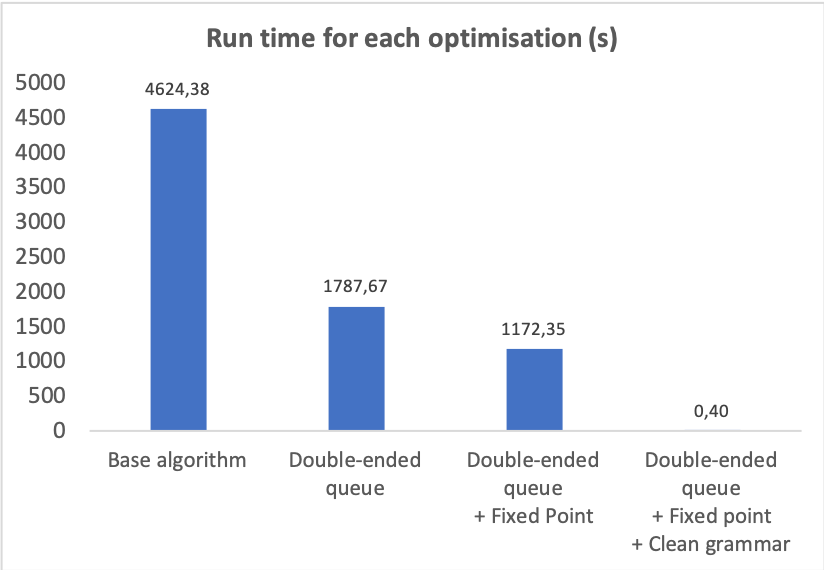
\includegraphics[height=4cm]{img/run_time}	\hspace*{2mm}
	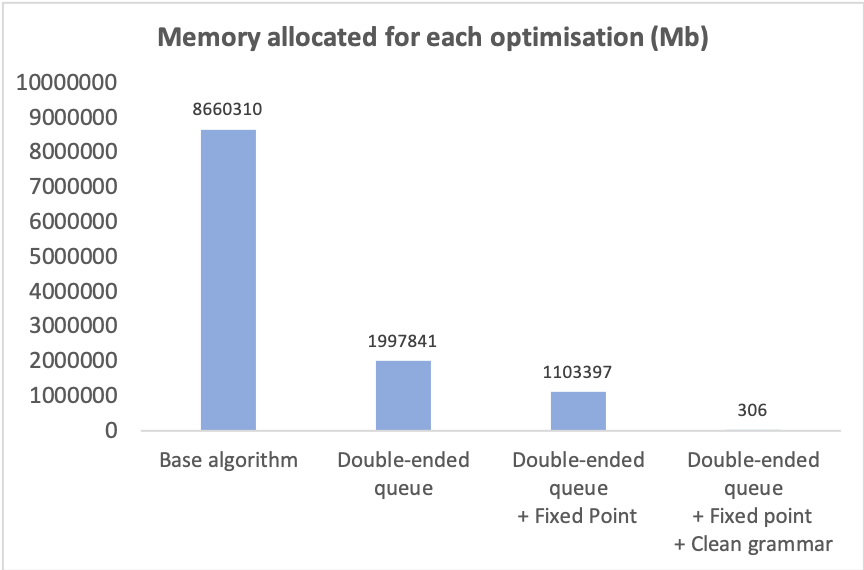
\includegraphics[height=4cm]{img/memory_alloc}
	\caption{Test results: running times (on the left) and
	memory allocated (on the right) checking the equivalence
	of context-free session types in 154 tests.}
	\label{fig:results}
\end{figure}

For the base algorithm, proposed in Listing~\ref{lst:algorithm}, we
obtained a running time of about 4624 seconds and
8,660,309 Mb memory allocated. From the moment we introduced the
optimizations the results improved remarkably: 
implementing a double-ended queue we reduced the running time to 1788 
seconds and the allocated memory to 1,997,841 Mb, by also
iterating the
simplification phase in the search for a fixed point we decreased these values
to a running time of 1172 seconds and 
allocated memory of 1,103,397 Mb. The 
combination of these enhancements with the clean grammar generation
exhibit an improvement in more than 1,000,000\% from the base case,
achieving a running time of 0.4 seconds and 306 Mb 
of memory allocated.

%iterating the
%simplification phase in the search for a fixed point allowed to reduce
%the running time to 110.35 seconds and the memory allocated to 164,745
%Mb, whereas the implementation of the double-ended queue allowed to
%reduce the running time to 18.45 seconds and the allocated memory to
%29,298. The combination of both exhibit an improvement on more than
%1,000,000\% from the base case, achieving an average of 0.04
%seconds for the running time and 62 Mb of allocated memory.

We should also highlight that, we run example~\eqref{ex:chaotic}
with the improved algorithm, in a battery of 100 runs, and obtained an
average running time of 0.008 seconds.

The heuristic we proposed actually circumvents the exponential complexity 
inherent to the expansion tree, thus allowing to obtain running times that 
are manifestly small and to use this algorithm as an integral 
part of a compiler, as we had intended from the beginning. 
%


%%% Local Variables:
%%% mode: latex
%%% TeX-master: "main"
%%% End:
